\lysh{14924}{4}

\begin{alist}
\item Το τριώνυμο $x^2 - x - 12$ έχει $\Delta = 1 - 4 \cdot (-12) = 1 + 48 = 49$ και δύο ρίζες άνισες, τις
$x_1 = \dfrac{-(-1) + \sqrt{49}}{2 \cdot 1} = \dfrac{1 + 7}{2} = 4$, $x_2 = \dfrac{-(-1) - \sqrt{49}}{2 \cdot 1} = \dfrac{1 - 7}{2} = -3$.
Το πρόσημο του τριωνύμου $x^2 - x - 12$ φαίνεται στον παρακάτω πίνακα

\begin{center}
\begin{tikzpicture}
\tikzset{t style/.style = {style = dashed}}
\tkzTabInit[color,lgt=3,espcl=2,colorC = maincolor!40,
colorL = maincolor!20,
colorV = maincolor!40]%
{$x$ / .8,$x^2 - x - 12$ /0.8}%
{$-\infty$,$-3$,$4$,$+\infty$}%
\tkzTabLine{ , $+$, z
, $-$ , z
, $+$ , }
\end{tikzpicture}
\end{center}

Δηλαδή $x^2 - x - 12 < 0$ για κάθε $x \in (-3, 4)$ και
$x^2 - x - 12 > 0$ για κάθε $x \in (-\infty, -3) \cup (4, +\infty)$.

\item Είναι $\pi > 3 \Leftrightarrow \pi + 9 > 12 \Leftrightarrow \dfrac{\pi + 9}{3} > 4$, οπότε με βάση το $\alpha)$ έχουμε ότι
\[\left(\dfrac{\pi + 9}{3}\right)^2 - \left(\dfrac{\pi + 9}{3}\right) - 12 > 0.\]

\item Η παράσταση $(\alpha + 3)^2 - (\alpha + 3) - 12$ είναι η τιμή του τριωνύμου για $x = \alpha + 3$ και για
να είναι αρνητική θα πρέπει:
\[-3 < \alpha + 3 < 4 \Leftrightarrow -6 < \alpha < 1 \Leftrightarrow \alpha \in (-6, 1).\]
\end{alist}

